\chapter{Results and Discussion}\label{ch:results}

\section{Results}\label{sec:results}

\begin{comment}
    SECTION IN PROGRESS
    This section should contain the results (mostly plots).  
    I think about the following suggested cases (as time allows):
    
    \begin{enumerate}
        \item  New suggested system, as a test case: Only one SQUID without periodic array, essentially as
        in Johansson, but with DCE radiation on both sides instead of only 1 side. This case has just one single $S$ matrix. 
        
        \item Now we embed the one SQUID from item 1 in a static periodic lattice, to see the effect of a band structure:
        Harmonic drive for only one SQUID: $\epsilon > 0$ for all SQUIDs, but $\epsilon_n^0 > 0$ only for one SQUID in the middle of the array. 
        
        \item Uniform harmonic drive, with $\epsilon_n^0 = \epsilon^0$ equal for all SQUIDs and $\varphi_n = 0$.
    
        \item Right-left symmetry breaking case:  
    $\epsilon_n^0 = \epsilon^0$ equal for all SQUIDs but $\varphi_1 = 0$, $\varphi_2 = 2 \pi / 3$, 
    $\varphi_3 = 2 * (2 \pi) / 3$, $\varphi_3 = 0$, and then repeated in 3-er blocks.
    This can also be written as $\varphi_n = n * (2 \pi) / 3$. 
    The super-transfer matrix will have the form $T^{(s)} = T^{(3)} T^{(2)} T^{(1)}$ where $T^{(s)}$ 
    is periodically repeated ("repeated unit cell for symmetry-breaking harmonic drive")
    
    \end{enumerate}
    
    \vspace{1cm}
    
    We use $\epsilon = 5$ as discussed.
\end{comment}
Below, we present the results of our analysis. We concentrate on output radiation (photon number density), as a function of frequency.

The band structure in our system can be tuned by changing the spatial distance $\ell$ between SQUIDs, as well as their Josephson energy $E_J^0$ (which corresponds to changing the strength of the potential at each site). Moreover, the harmonic drive of the SQUIDs generating the DCE radiation can be tuned in terms of the drive frequency $\Omega$, amplitude $\delta E_{J,\,n}$, and phase $\varphi_n$, where the latter two parameters can be modulated for each SQUID $n$ in the periodic array individually. This allows us to go one step further than regular photonics, where the band structure can be engineered, and further control spectral and spatial properties of the dynamical Casimir light emitted making our proposed lattice architecture quite versatile. 

Unless specified, the input parameters for the calculations are (unitless) drive frequency $\Omega= 12$, lattice parameter $\epsilon = 5$, modulation amplitude $\delta \epsilon = \epsilon/4$.


\newpage

\section{Preliminary results: One SQUID, both sides allowed}\label{sec:results_both_sides}
%
We present here a preliminary result, as a test that our calculation algorithm produces sensible physical results. Below, in Fig. \ref{fig:naked_SQUID}, we show the output radiation emitted by a single SQUID, allowing the field to propagate on both sides of the SQUID site. This is in contrast to previous work \cite{Johansson2009}, from which we borrow input parameters. We obtain a similar result, producing the distinctive one-mirror parabolic DCE shape described in \cite{Lambrecht1996}. The one important distinction is that, by allowing the field to propagate on both sides of the mirror (effectively making the mirror semi-transparent as opposed to perfectly reflecting), radiation travels away from the mirror on both sides. A slightly higher overall photon count is produced as well. 
%
We first show, as a preliminary result, the radiation emitted by a single SQUID, where we allow the field to propagate on both sides of the SQUID (as opposed to the work in \cite{Johansson2010}, where the field can only propagate to one site of the SQUID).  
%
\begin{figure}[h]
    \centering
    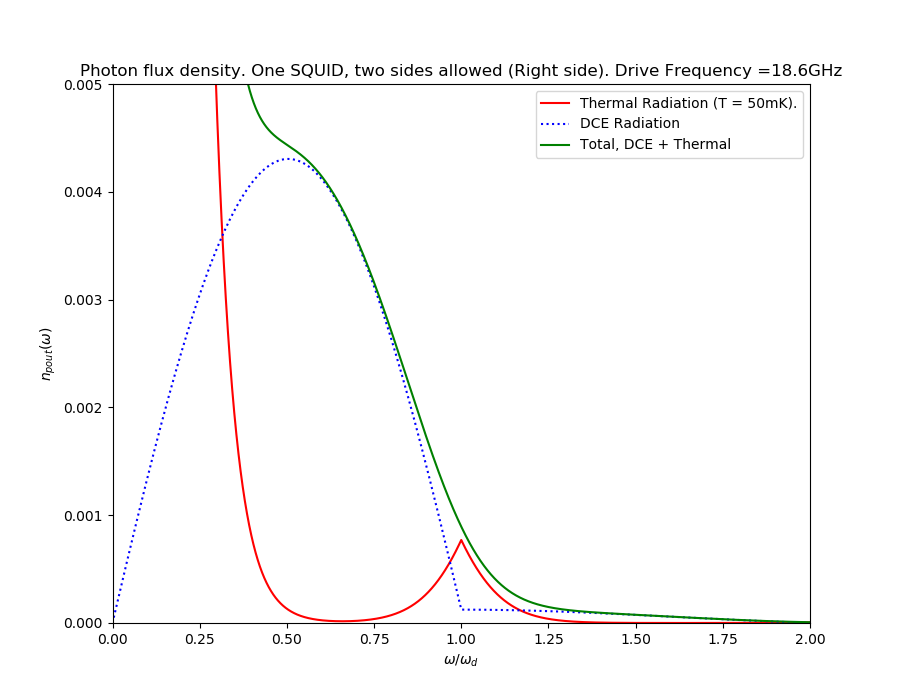
\includegraphics[width=0.9\textwidth, keepaspectratio]{figures/results/Naked_SQUID_right.png}
    \caption{Output radiation for one single semi-transparent SQUID. We allow both sides of the SQUID to have incoming/outgoing radiation. Horizontal axis is normalized with drive frequency $\omega_d$. Output radiation is symmetric.}
    \label{fig:naked_SQUID}
\end{figure}
%

\newpage
\section{Results: One SQUID embedded in lattice}\label{sec:results_one_active}
We now discuss results of our own model for a periodic SQUID lattice. Forbidden regions (see Section \ref{subsec:kpsol}) are shown in green. For these regions, no radiation (DCE or thermal) travels outside of the lattice. Detectable radiation is produced only within allowed regions.

For the following figures (\ref{fig:one_SQUID_active}-\ref{fig:one_SQUID_active_e_14_T_50}), only one SQUID is drive at a frequency $\Omega =12$, in a periodic lattice with different lattice parameters $\epsilon$. Different radiation patters emerge by changing the drive frequency and lattice parameter. Figure \ref{fig:one_SQUID_active}, shows the radiation produced by one single driven SQUID in a lattice $\epsilon=5$ which corresponds to physical lattice separation of about 2.21mm.
%
\begin{figure}[h]
    \centering
    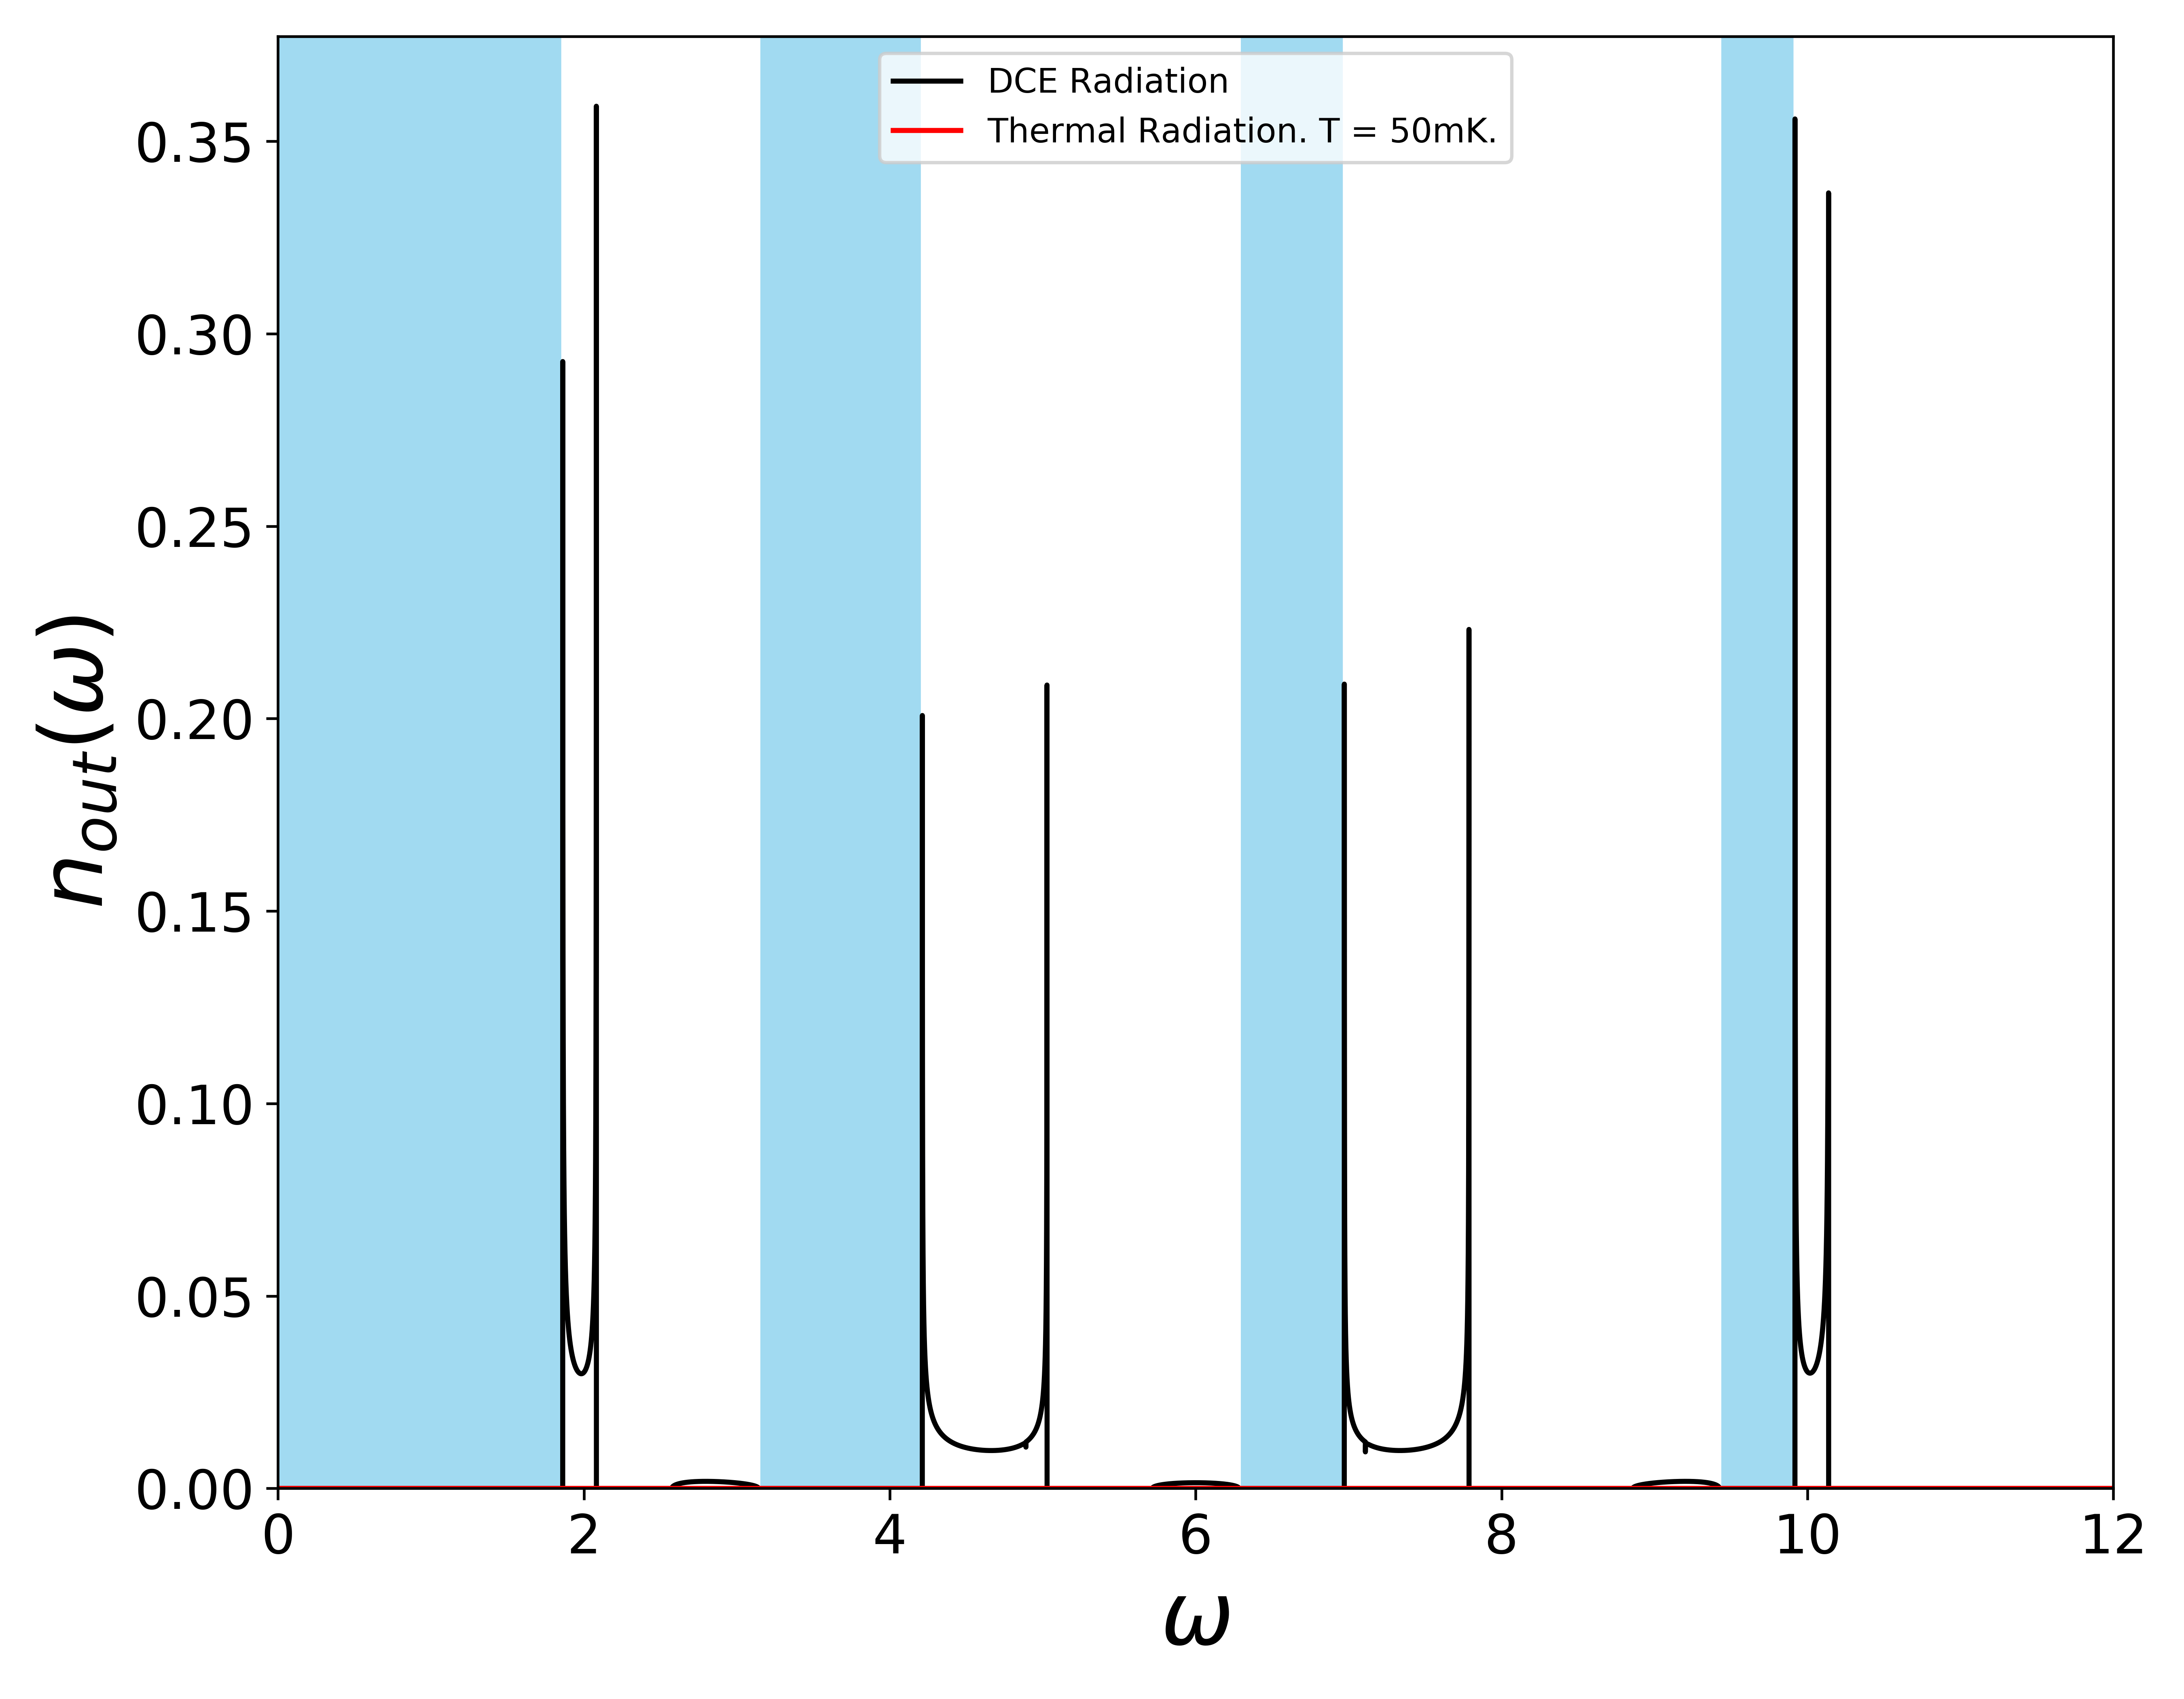
\includegraphics[width=\textwidth, keepaspectratio]{figures/results/one_SQUID_active.png}
    \caption{Output radiation for one single driven SQUID embedded in lattice with 50 static SQUIDs to either side. Unitless variables used: $\Omega=12$, $\epsilon=5$.}
    \label{fig:one_SQUID_active}
\end{figure}
%
\newpage

The radiation pattern changes dramatically compared to the one for a single SQUID in "free space" (see Fig. \ref{fig:naked_SQUID}). This is due to the presence of allowed and forbidden regions,as well as the change in the boundary condition due to the properties of Bloch functions, and the shape of the ground states of the field excited by the perturbation of such boundary conditions.

%
\begin{figure}[h]
    \centering
    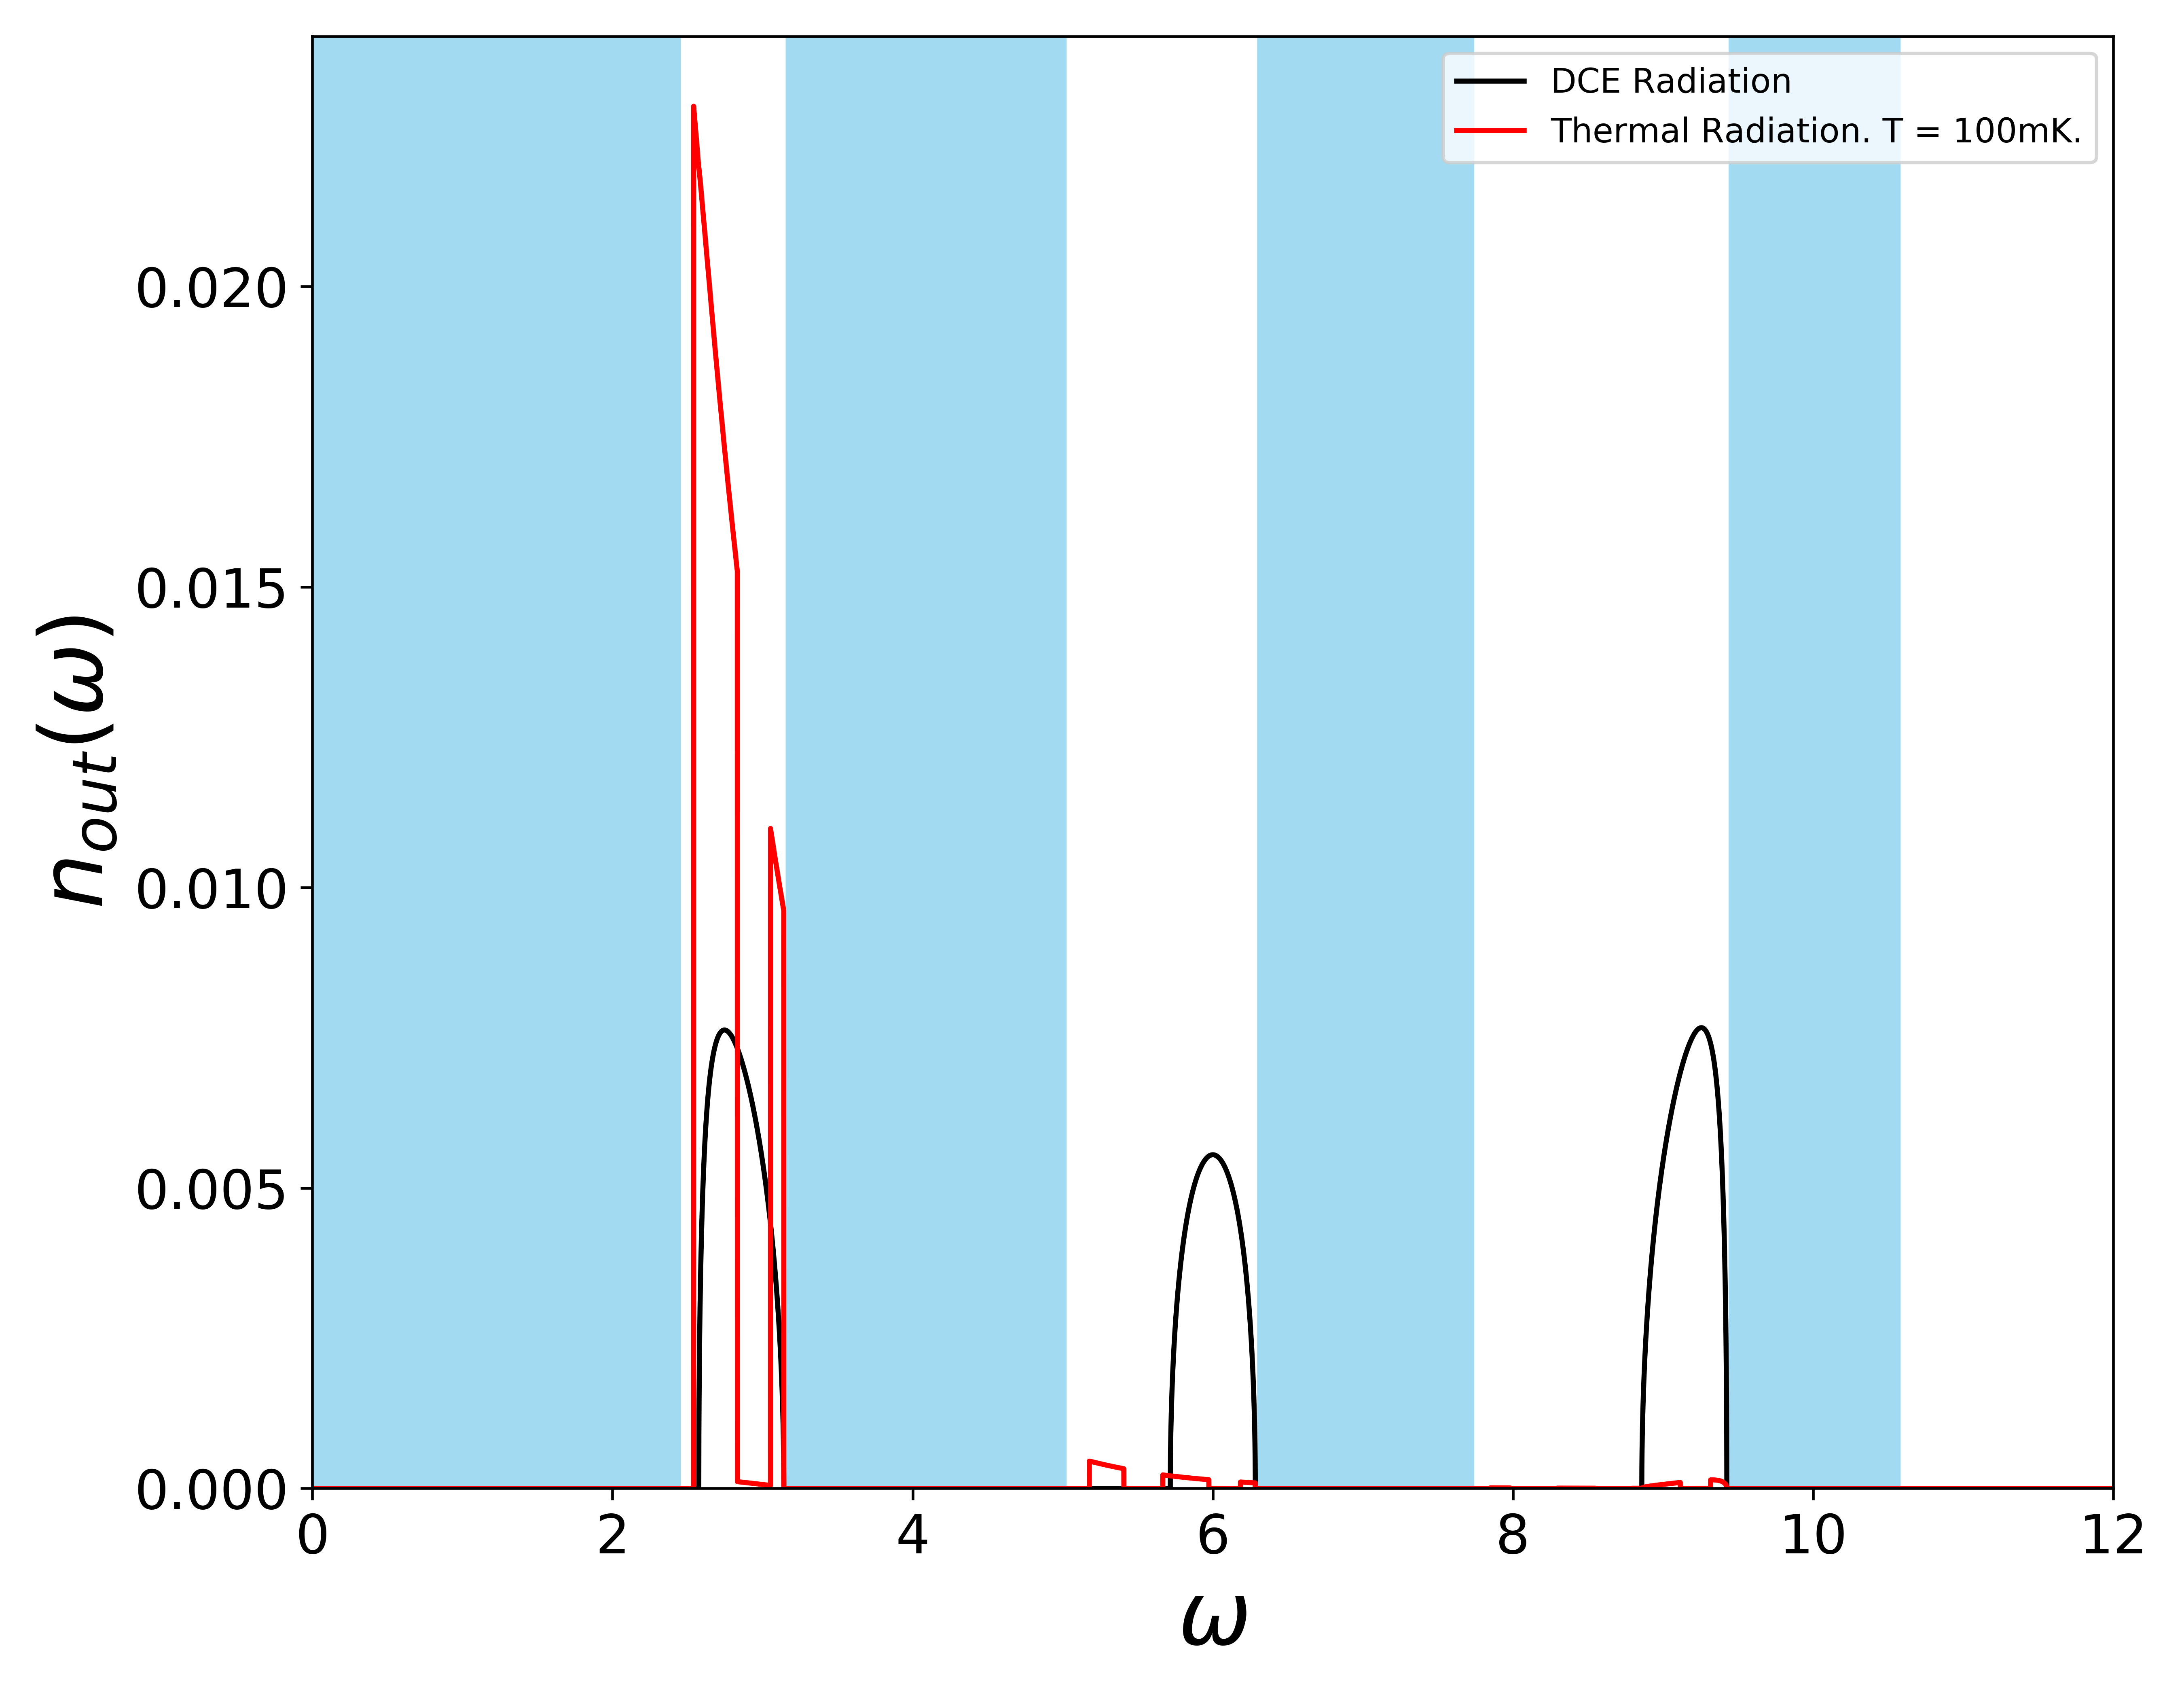
\includegraphics[width=\textwidth, keepaspectratio]{figures/results/one_SQUID_active_epsilon_14_100mK.png}
    \caption{Output radiation for one single driven SQUID embedded in lattice. Unitless variables used: $\Omega=12$, $\epsilon=14$. A different band structure shows thermal contributions to the radiation. Temperature = 100mK.}
    \label{fig:one_SQUID_active_e_14_T_100}
\end{figure}
%
Note that the presence of forbidden regions, particularly the region before the first allowed band, make it so the thermal radiation is filtered out. Since the input thermal radiation follows an inverse exponential relation for low frequencies (see Fig. \ref{fig:naked_SQUID}), the first forbidden region absorbs most of the thermal radiation. By changing the structure of the lattice to $\epsilon = 14$, the presence of thermal radiation can be observed, as well as well as different features in the DCE radiation.
%
\begin{figure}[h]
    \centering
    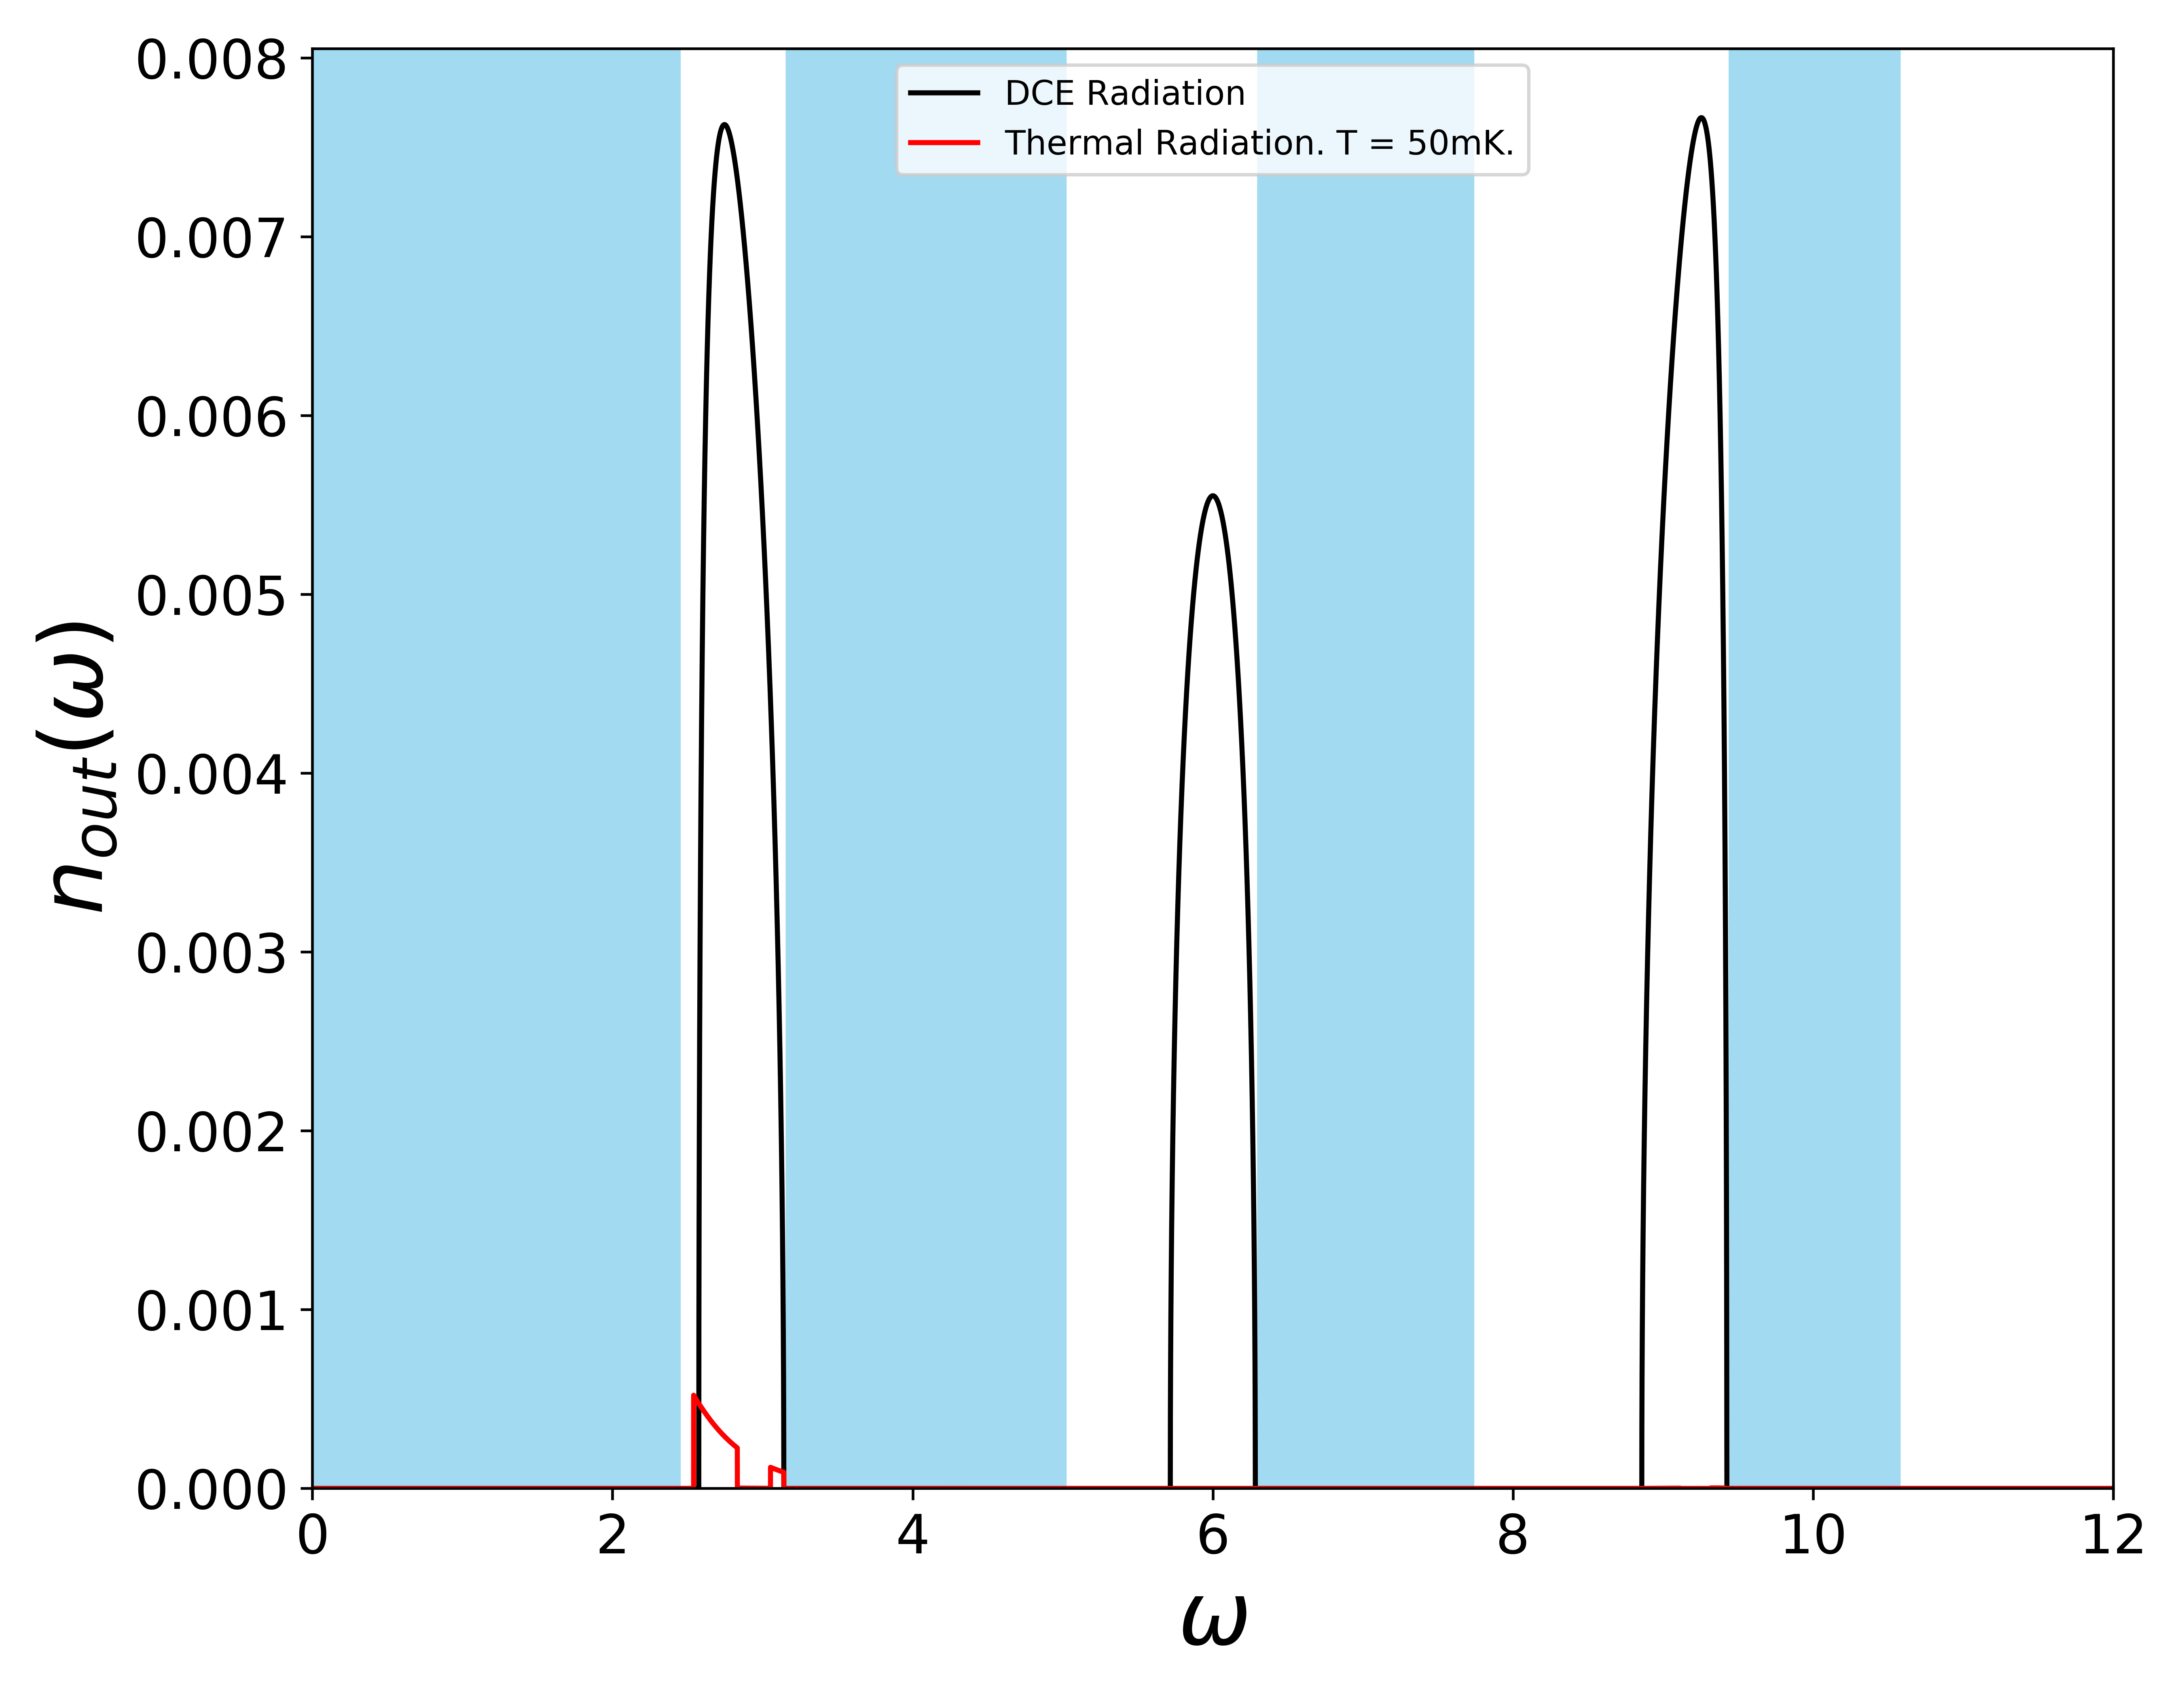
\includegraphics[width=\textwidth, keepaspectratio]{figures/results/one_SQUID_active_epsilon_14.png}
    \caption{Output radiation for one single driven SQUID embedded in lattice. Unitless variables used: $\Omega=12$, $\epsilon=14$. A different band structure shows thermal contributions to the radiation. Temperature = 50mK.}
    \label{fig:one_SQUID_active_e_14_T_50}
\end{figure}
%

\newpage

Figure \ref{fig:one_SQUID_active_e_14_T_50}, shows the distinct features of DCE radiation when compared to a different band structure (see Fig. \ref{fig:one_SQUID_active}). Here, the radiation is closer to the familiar single-SQUID parabolic shape. Note how the features of DCE radiation are not localized in one allowed region but instead cover multiple regions. These likely correspond to higher order scattering as the Bloch waves are scattered by multiple active SQUIDs.

\newpage
\section{Results: All SQUIDs embedded in lattice}\label{sec:results_all_active}

Some text about all SQUIDS.

\begin{figure}[h]
    \centering
    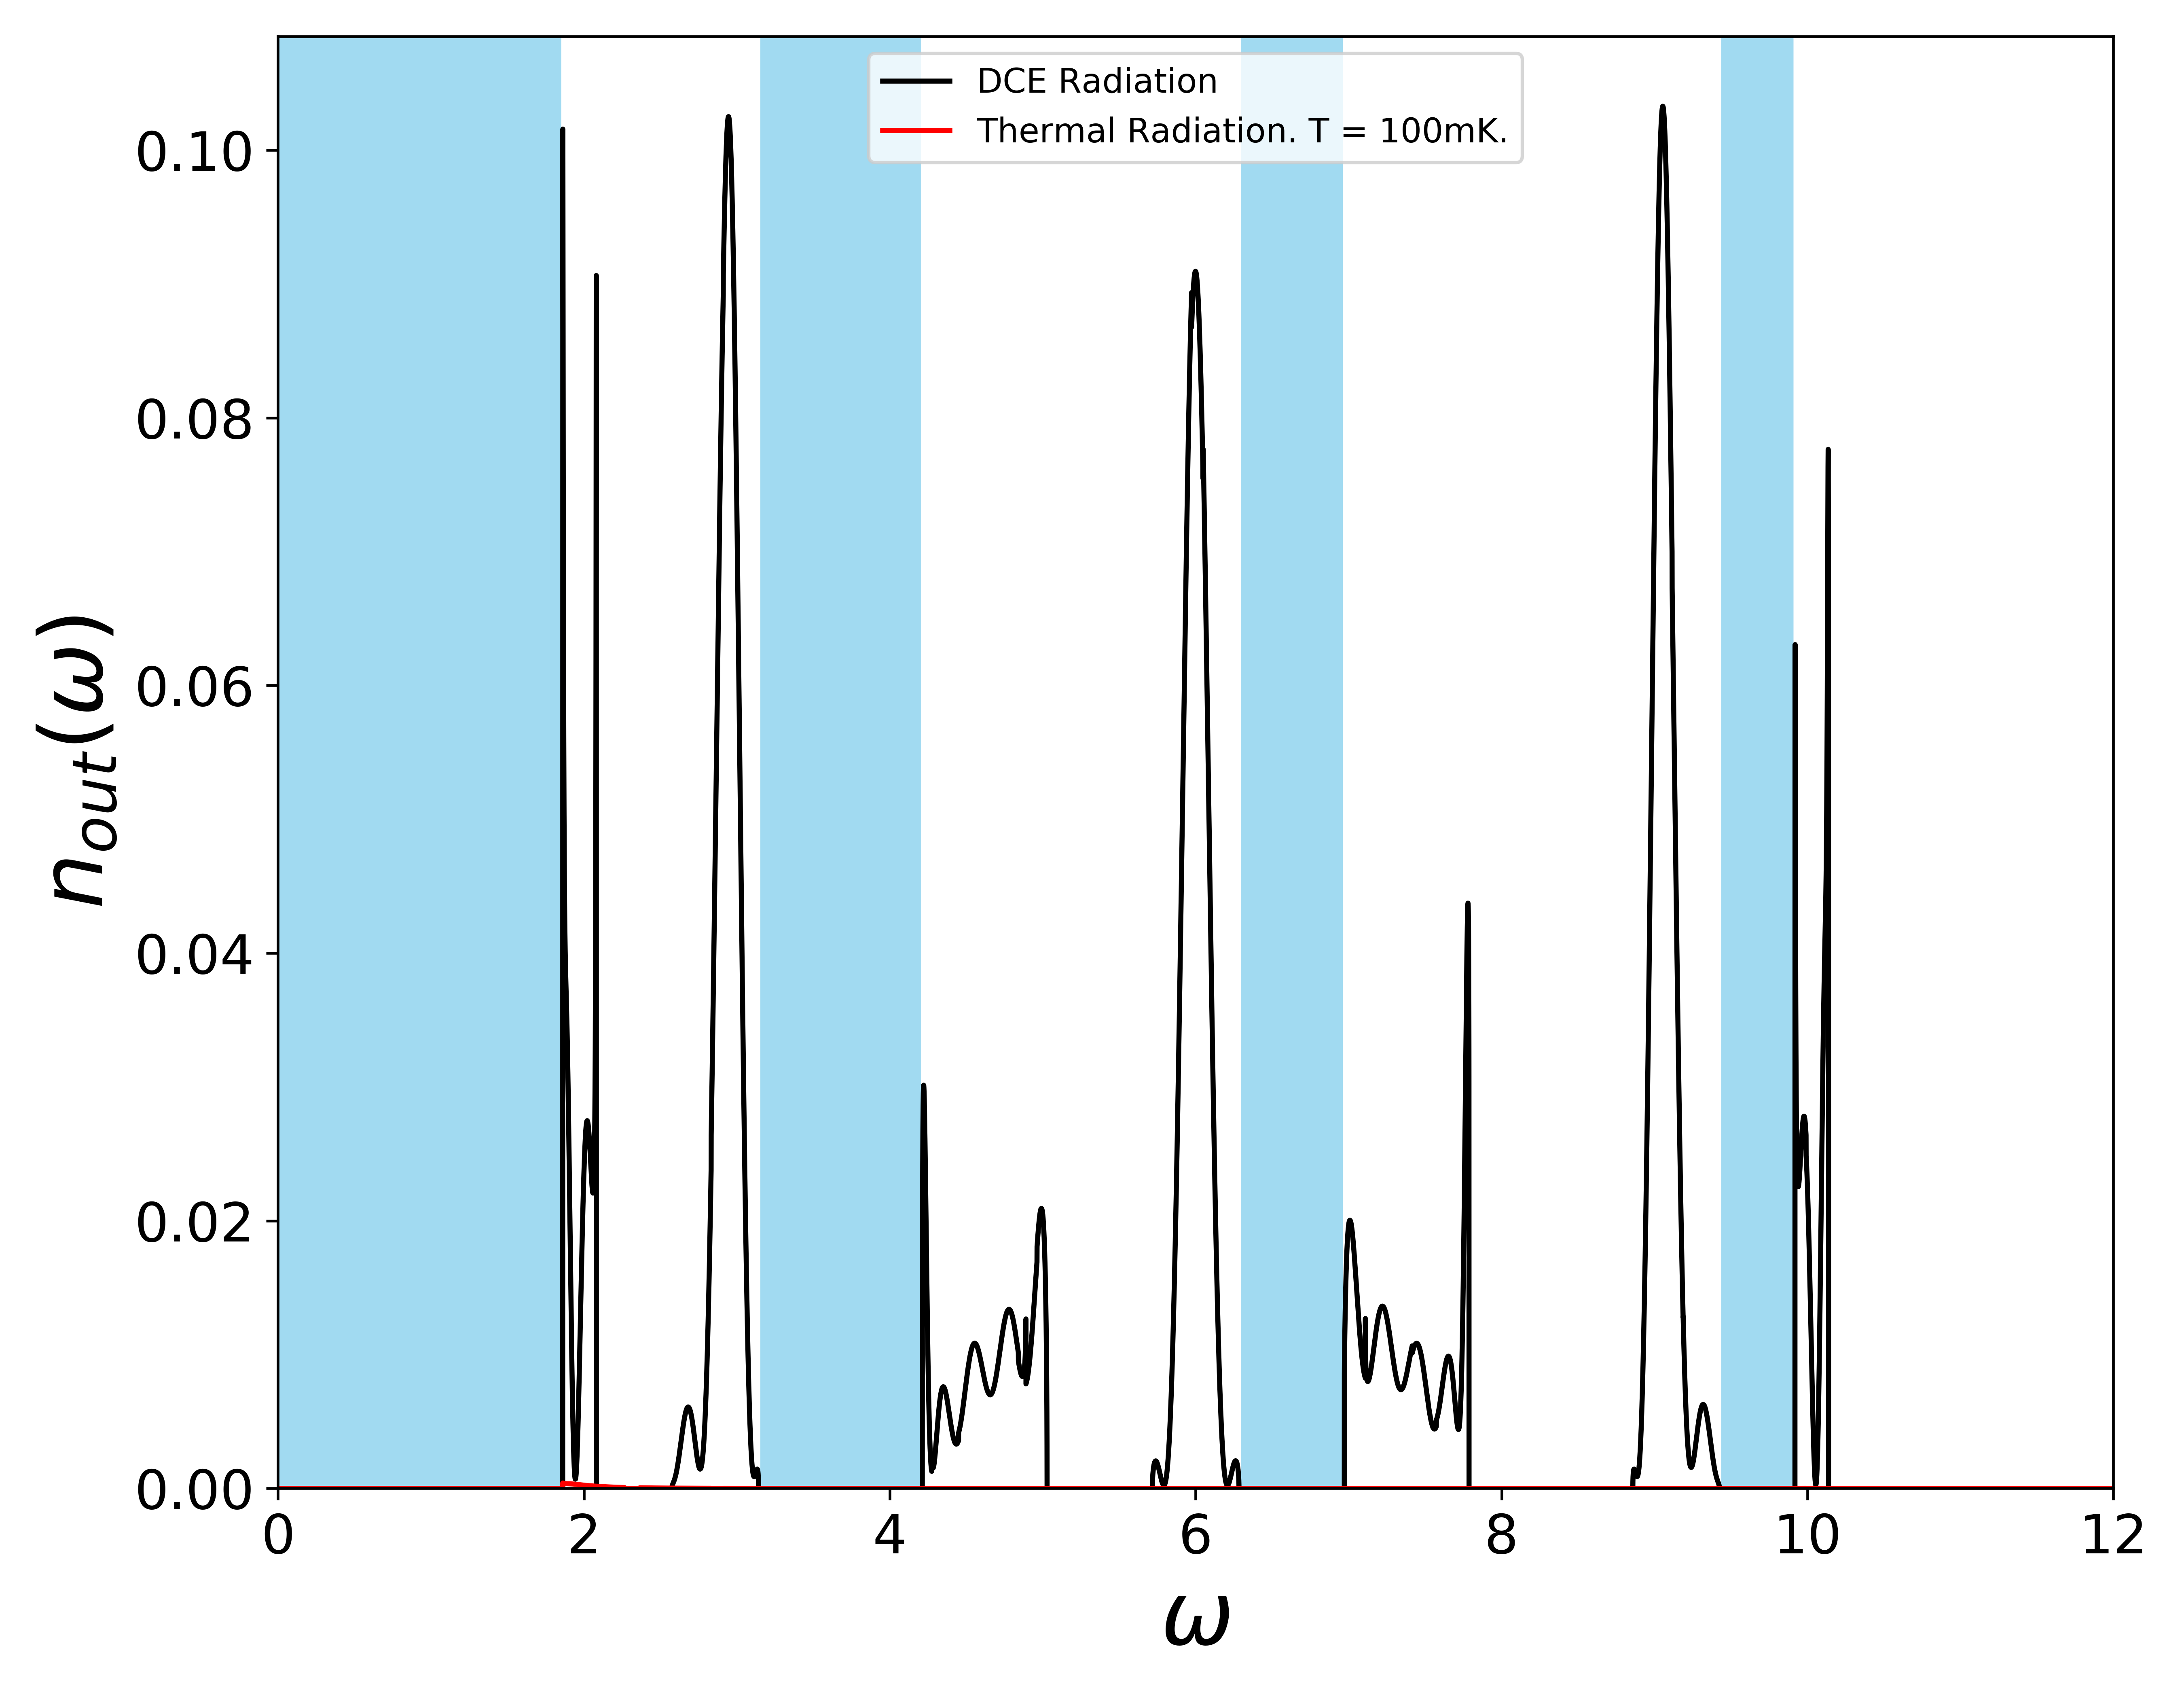
\includegraphics[width=\textwidth, keepaspectratio]{figures/results/10_SQUIDs_active.png}
    \caption{Output radiation for lattice of 10 driven SQUIDs. Unitless variables used: $\Omega=12$, $\epsilon=5$. Complex radiation patterns arise when all SQUIDs are active.}
    \label{fig:10_SQUIDs_active}
\end{figure}
%
\begin{figure}[h]
    \centering
    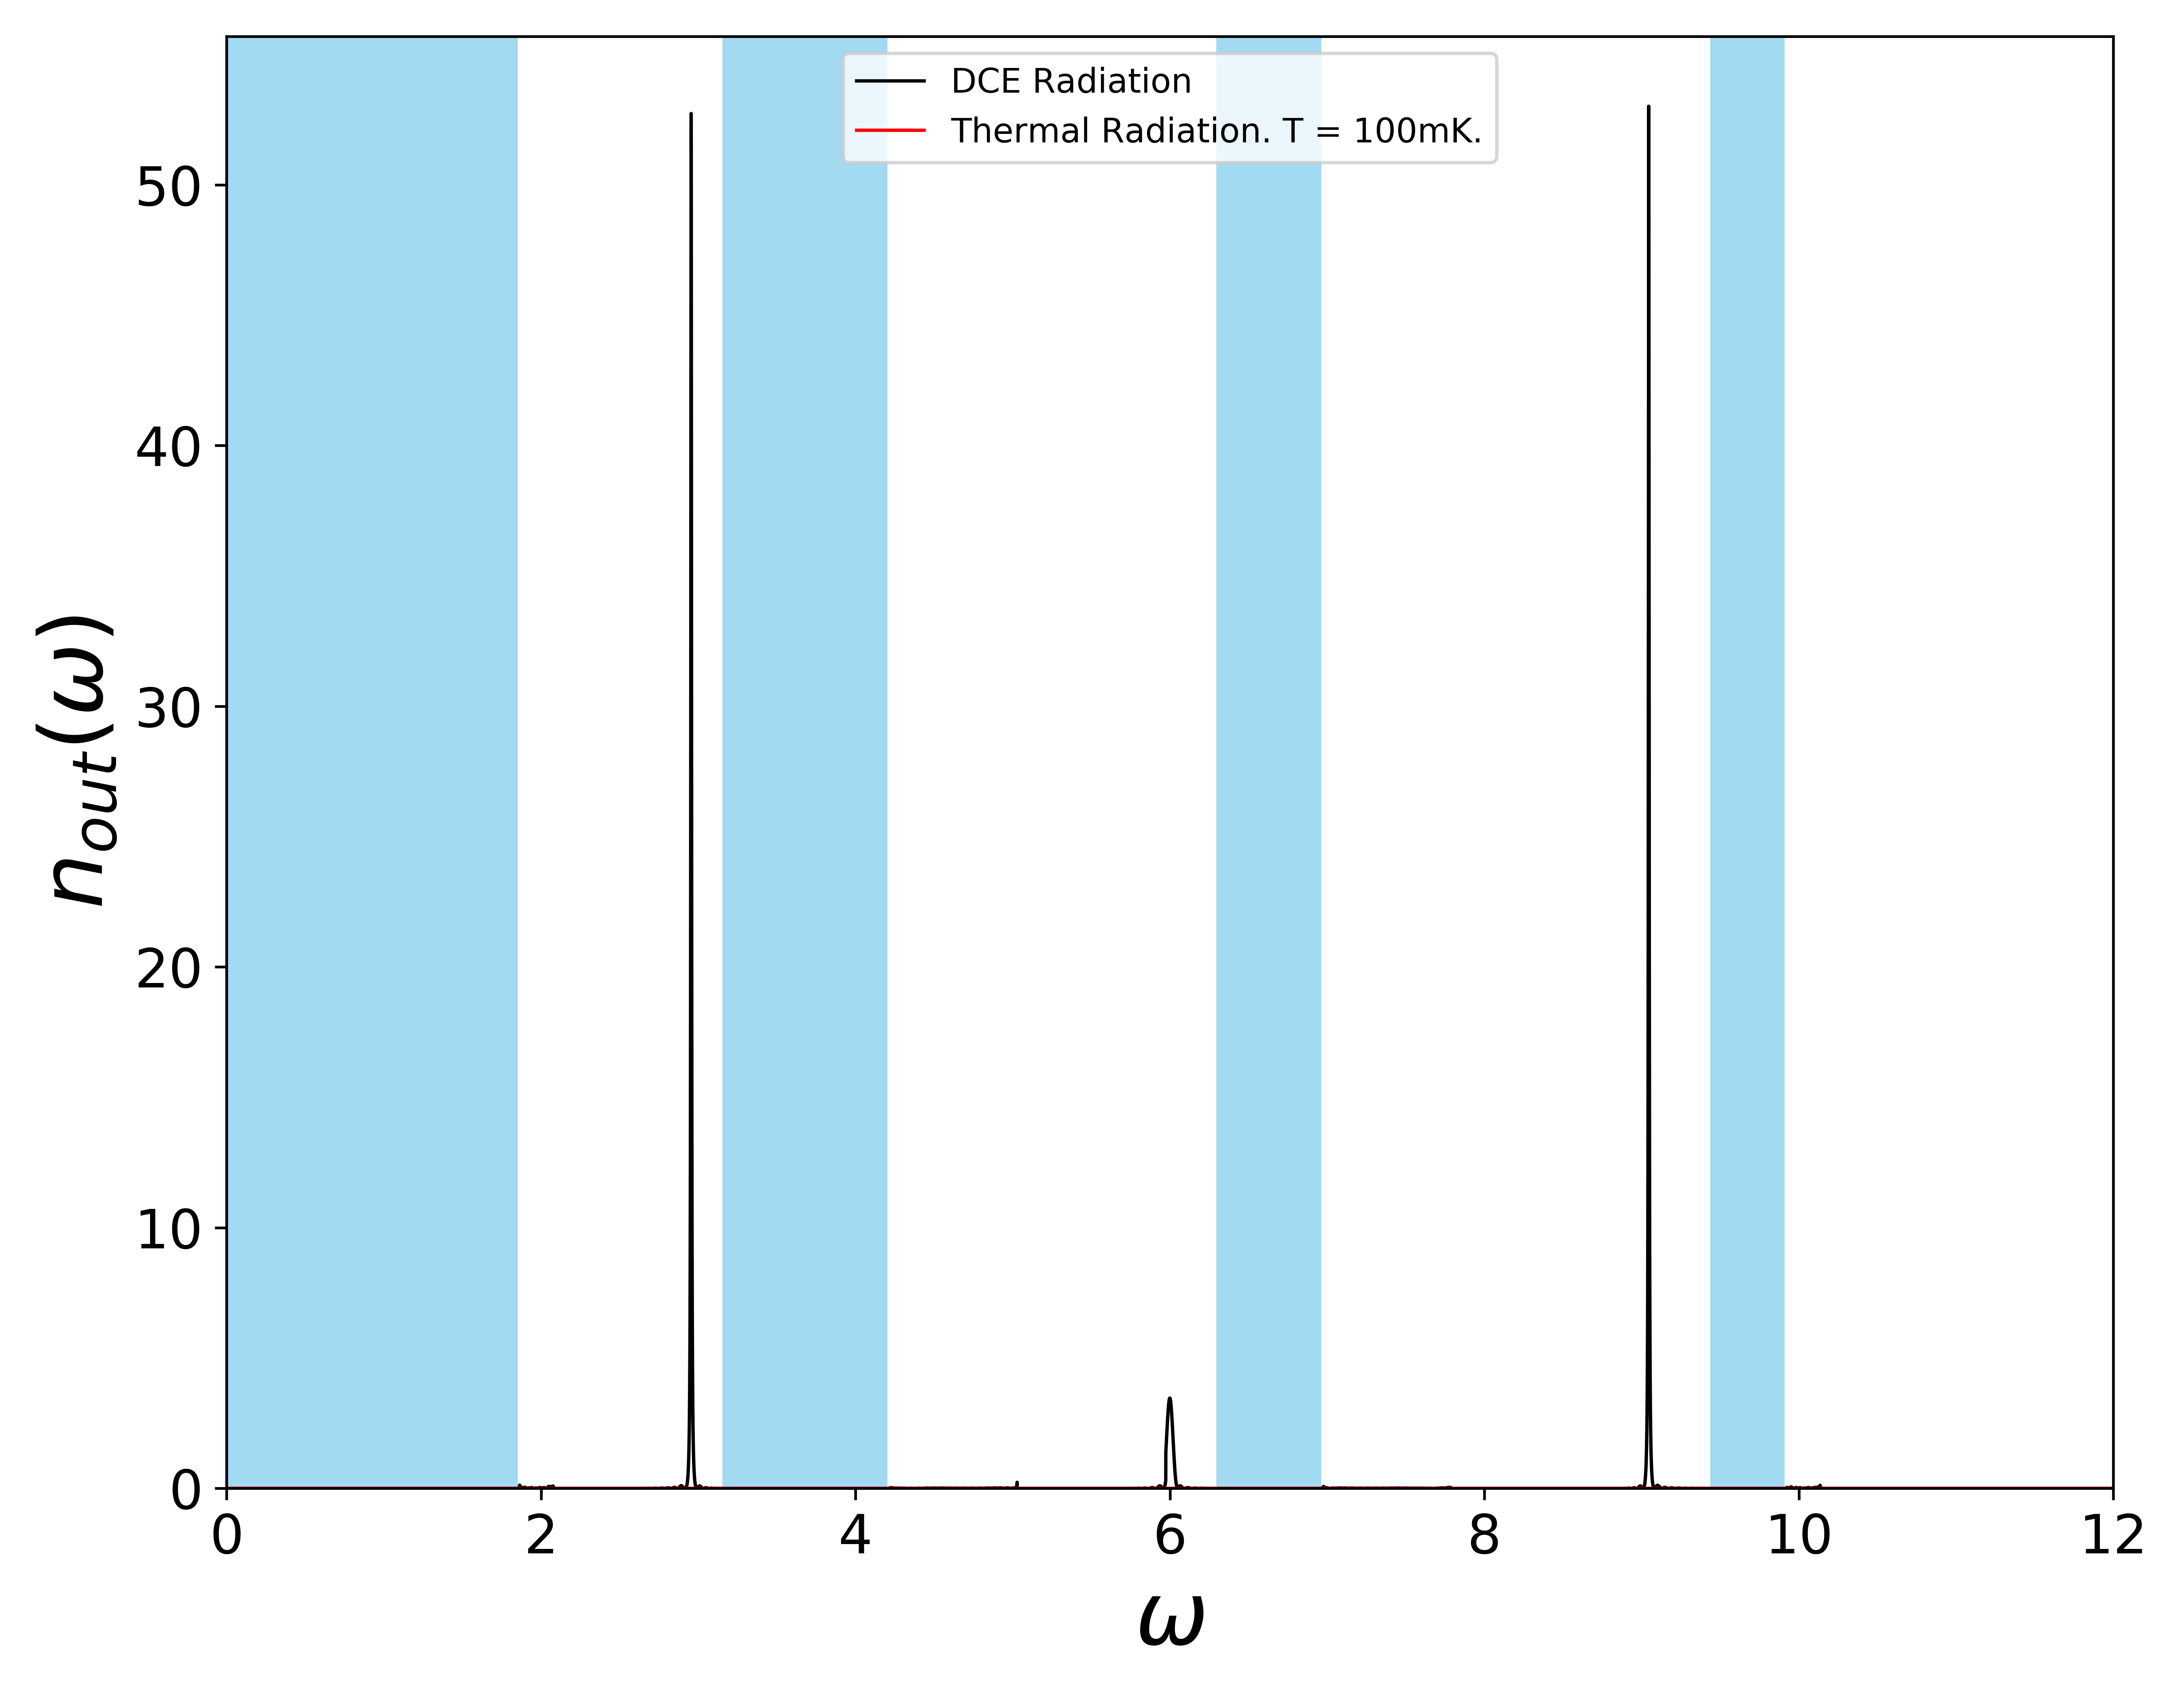
\includegraphics[width=\textwidth, keepaspectratio]{figures/results/50_SQUIDs_active.png}
    \caption{Output radiation for lattice of 50 driven SQUIDs. Unitless variables used: $\Omega=12$, $\epsilon=5$.}
    \label{fig:50_SQUIDs_active}
\end{figure}
%
\begin{figure}[h]
    \centering
    \includegraphics[width=\textwidth, keepaspectratio]{figures/results/100_SQUIDs_active.png}
    \caption{Output radiation for lattice of 100 driven SQUIDs. Unitless variables used: $\Omega=12$, $\epsilon=5$.}
    \label{fig:100_SQUIDs_active}
\end{figure}
%
\begin{figure}[h]
    \centering
    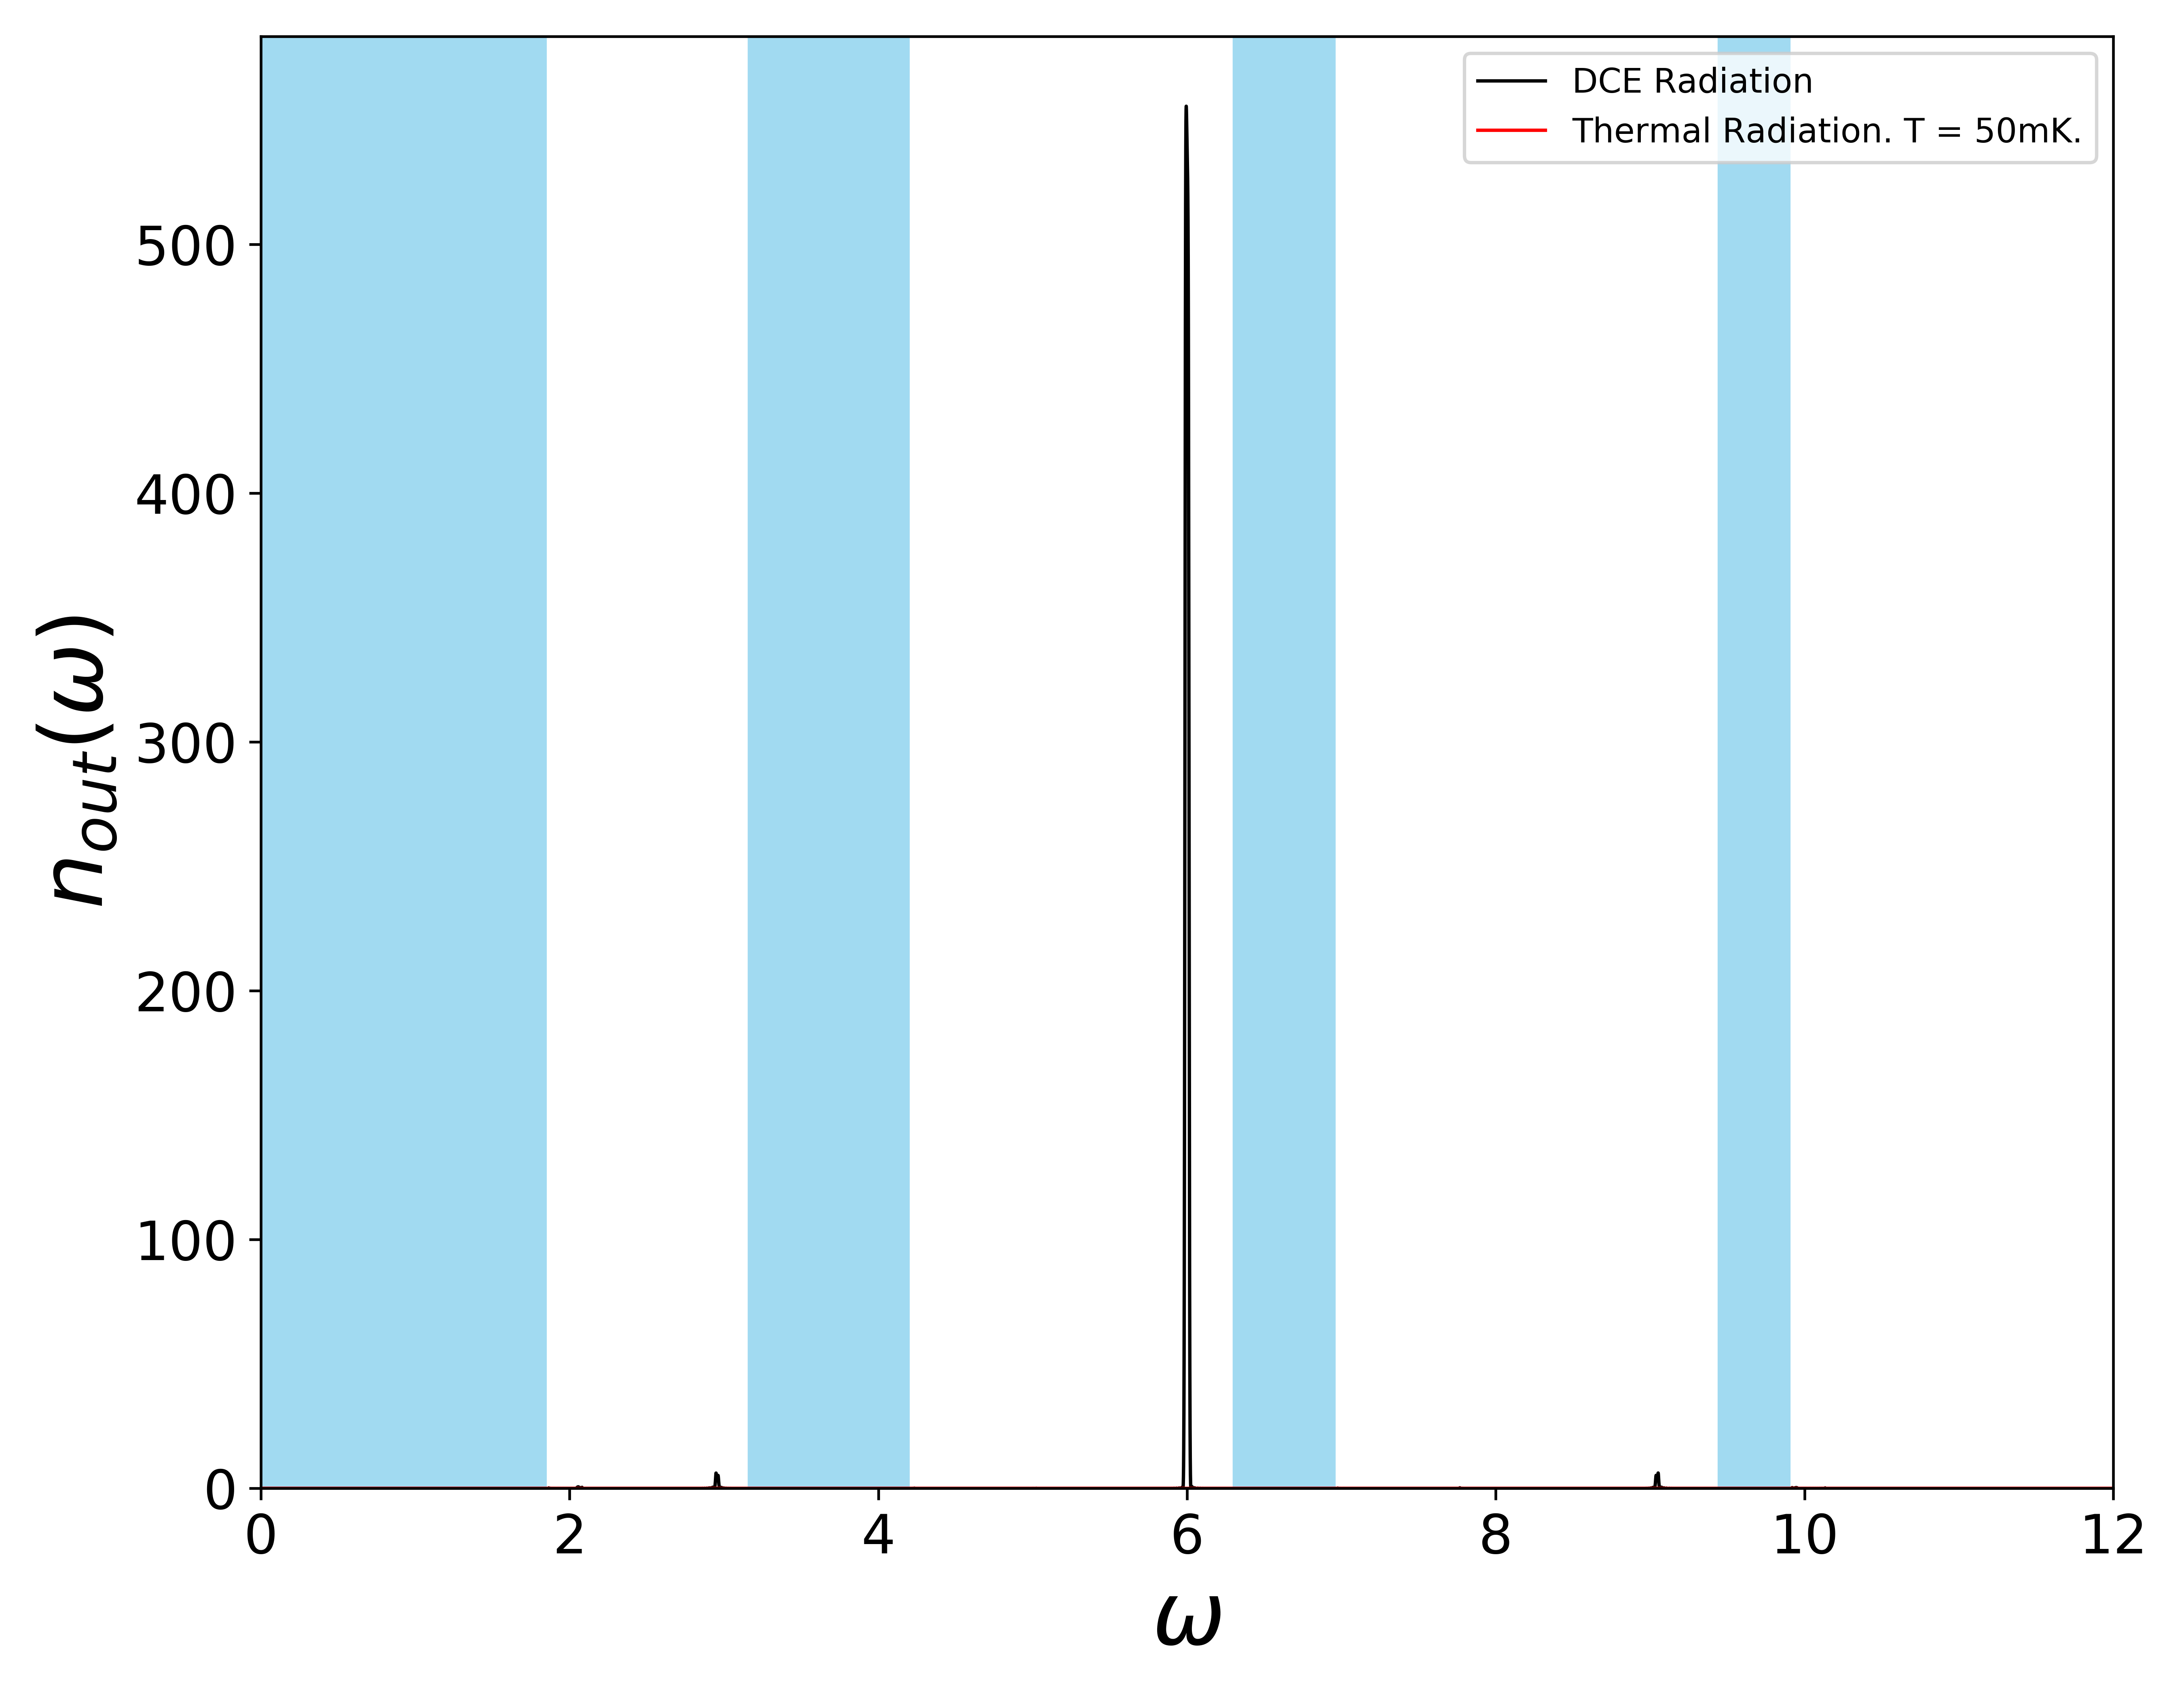
\includegraphics[width=\textwidth, keepaspectratio]{figures/results/150_SQUIDs_active.png}
    \caption{Output radiation for lattice of 150 driven SQUIDs. Unitless variables used: $\Omega=12$, $\epsilon=5$.}
    \label{fig:150_SQUIDs_active}
\end{figure}
%
\section{Results: Spatial symmetry breaking}\label{sec:results_symmetry_breaking}
%

\begin{comment}

\begin{figure}[h]
    \centering
    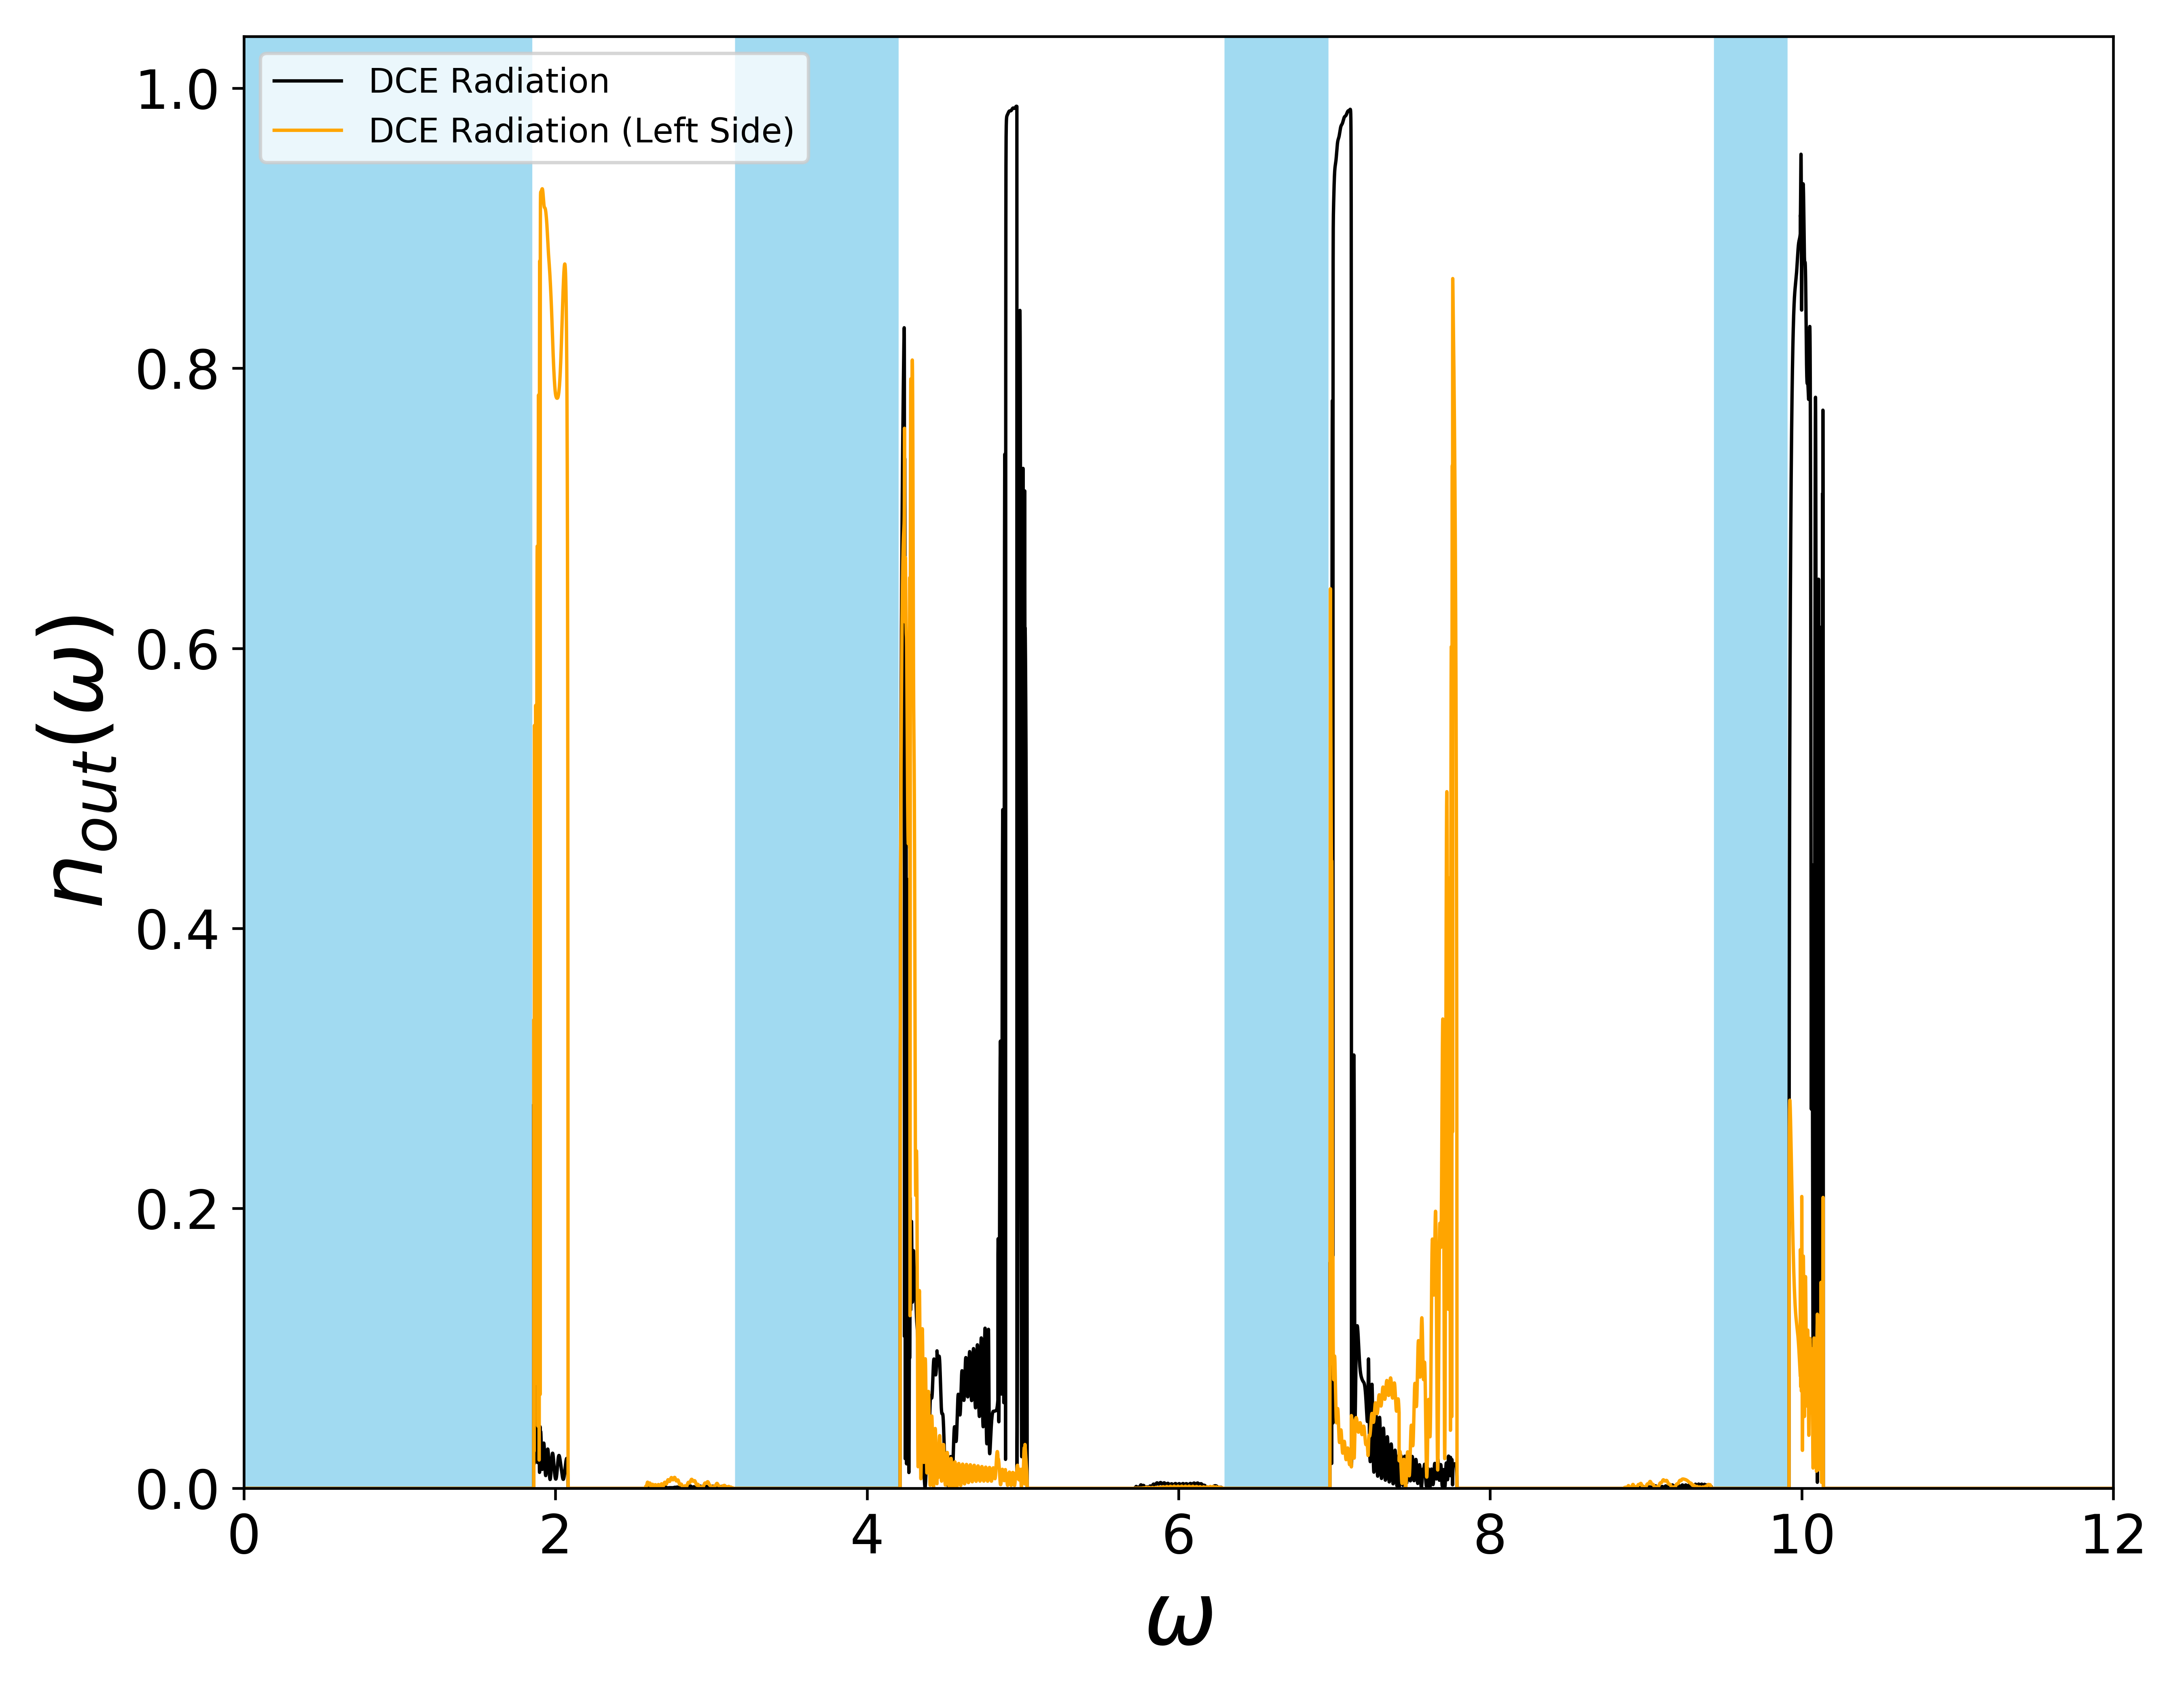
\includegraphics[width=\textwidth, keepaspectratio]{figures/results/phase_shift_2pi_3_both.png}
    \caption{Output radiation for lattice of 100 SQUIDs driven out of phase. Introducing a phase shift factor breaks the spatial symmetry of the lattice. Here, each SQUID is driven at a phase difference of $\frac{2\pi}{3}$ with respect to the previous SQUID, effectively creating a new 3-SQUID unit cell.}
    \label{fig:phase_2pi_3_right}
\end{figure}
%
\begin{figure}[h]
    \centering
    \includegraphics[width=\textwidth, keepaspectratio]{figures/results/phase_2pi_3_left.png}
    \caption{Output radiation for lattice of 100 SQUIDs driven out of phase. Introducing a phase shift factor breaks the spatial symmetry of the lattice. Phase factor = $\frac{2\pi}{3}$.}
    \label{fig:phase_2pi_3_left}
\end{figure}
%
\begin{figure}[h]
    \centering
    \includegraphics[width=\textwidth, keepaspectratio]{figures/results/phase_2pi_5_right.png}
    \caption{Output radiation for lattice of 100 SQUIDs driven out of phase. Phase factor = $\frac{2\pi}{5}$, 5-SQUID unit cell.}
    \label{fig:phase_2pi_5_right}
\end{figure}
%
\begin{figure}[h]
    \centering
    \includegraphics[width=\textwidth, keepaspectratio]{figures/results/phase_2pi_5_left.png}
    \caption{Output radiation for lattice of 100 SQUIDs driven out of phase. Phase factor = $\frac{2\pi}{5}$, 5-SQUID unit cell. Drastic difference in the left/right output radiation.}
    \label{fig:phase_2pi_5_left}
\end{figure}
\end{comment}

We find a rich interplay between the band structure of the lattice, the harmonic drive of the SQUIDs, and the DCE photon-flux density, which thus allows us to control, guide, and manipulate DCE radiation. 
